\documentclass[letterpaper,12pt,fullpage]{article}

\usepackage[left=1in,right=1in,top=1in,bottom=1in]{geometry}
\usepackage{cite}
\usepackage{graphicx}
% \usepackage[dvips]{graphicx}
% \usepackage{epsfig} % for postscript graphics files
  % \graphicspath{{../eps/}}
% \DeclareGraphicsExtensions{.eps}
\usepackage{amsmath}
\usepackage{amssymb}
%\usepackage[cmex10]{amsmath}
%\usepackage{array}
%\usepackage{mdwmath}
%\usepackage{mdwtab}
%\usepackage{eqparbox}
\usepackage[tight,footnotesize]{subfigure}
%\usepackage[caption=false]{caption}
%\usepackage[font=footnotesize]{subfig}
%\usepackage{fixltx2e}
%\usepackage{stfloats}
\PassOptionsToPackage{hyphens}{url}\usepackage{hyperref}
\usepackage{hyperref}

% correct bad hyphenation here
%\hyphenation{op-tical net-works semi-conduc-tor}

\input latex-commands

\newcommand{\shrinkfig}{\def\baselinestretch{1.0}\small} % 0.9 okay
\newcommand{\shrink}{\def\baselinestretch{1.1}\small} % 0.97 % 0.95 okay

\begin{document}

\title{Estimating Operator Intent\\
(Draft 4.0)}

\author{Alex Ansari, Christopher G. Atkeson, Howie Choset, and Matthew Travers\\
Carnegie Mellon University}

\maketitle

\section{Executive Summary}

\begin{enumerate}
\item
We recommend using a Bayesian {\bf (probabilistic) framework}
for intent recognition and prediction.
\item
We recommend developing an intent prediction system that can use
as {\bf many sensors and measurements} of the operator as possible.
\item
We seriously consider {\bf implanting devices and markers} in operators.
\item
We recommend each exoskeleton controller
to be used by and {\bf optimized for a single operator.}
A substantial investment in capturing the operator's normal behavior,
operator training and learning, and controller customization should be made.
\end{enumerate}

\section{Clickable web links}

The web links (URLs) below can be clicked on to view, if your PDF viewer/browser supports that. On our browsers you actually have to click on the black
part of a letter, not just in the blue box (if present).

\section{Scope: What is this paper about?}

This paper surveys state of the art technology to recognize
and predict exoskeleton
operator intent.
A companion paper surveys current operator/exoskeleton interfaces.\\
\url{http://www.cs.cmu.edu/~cga/exo/survey.pdf}

The focus is on intent estimation that allows a
highly trained and top percentile athletic 
operator to carry a payload that weighs approximately the same amount
as the operator. We envisage these types of exoskeletons to be useful
in carrying protective and safety equipment for SWAT teams, police,
firefighters, and soldiers. 

We focus this survey on intent estimation for highly dynamic 
lower body tasks (standing, walking,
running, jumping, kicking, dodging, ...).
We do not survey intent estimation for manipulation. 

A future white paper could discuss how intent estimation could be 
made easier with outward facing
superhuman perception (sensing beyond human capabilities
or modalities) such as cameras looking out all over the skin
of the suit (whole-body vision), or whole-body 
infrared vision of the situation.

A future white paper could discuss how intent estimation could be 
made easier with inward facing superhuman perception,
such as implanted markers and devices, as well as continuous
operator imaging such as reflective and/or transmissive ultrasound
tracking tissue parameters or implanted markers.

Predictive models of human motion, a major topic of robot learning from\\
observation/demonstration/imitation and computer animation,
could be the subject of a future white
paper.\\
%~\cite{IEEE06913830}
\url{http://ieeexplore.ieee.org/xpl/login.jsp?tp=&arnumber=6913830}\\
\url{http://www.ri.cmu.edu/publication_view.html?pub_id=7891}

\section{Introduction: Our point of view}

{\bf What is intent estimation?}
The further in the future the control system can predict what the operator
is going to do, the easier it is to control the exoskeleton. One way
to think about estimating operator intent is to imagine you are in
a hand-to-hand fight (such as various forms of martial arts)
and you want to predict your opponent's next move.
You can also think about playing poker. What ``tells'' does the opponent
have?
You are allowed to instrument your opponent. What sensors would you use?
How would you interpret the sensors?

Here is an example of a robot seeing and moving faster than a human, and
consistently beating a human opponent in rock-paper-scissors.\\
\url{https://www.youtube.com/watch?v=Qb5UIPeFClM&feature=player_embedded}

\section{Who is the customer of intent predictions?}

One customer of intent estimation is an exoskeleton control system.
Other possible customers are online operator situation awareness,
cognitive assistance
and physical guidance;
command and squad visualization, situation awareness,
coordination, and cognitive assistance;
after-action reports; and new operator training and
operator learning from practice and coaching,
We will focus on exoskeleton control in this paper.

\section{What is the output of intent estimation?}

There are several possible outputs of intent estimation of use to the
exoskeleton control system.
Estimates and predictions could be actual values at the current time or at
future times, probability distributions for
values at various times such as Gaussians or multi-modal distributions 
such as mixtures of Gaussians, or probability distributions for trajectories
of values, supporting non-Markov models of processes such as libraries
of behaviors.

\subsection{Operator state (joint positions and velocities)}

It is useful to estimate the full state of the operator in terms
of joint positions and velocities.

\subsection{Operator-exoskeleton force}

One possible output of intent estimation is an estimate of current
and predicted future forces between the operator and the exoskeleton.

\subsection{Desired movement trajectory}

Exoskeleton model-based control systems based on inverse dynamics often
can make use of an estimate of the current desired acceleration.
Predictions can be in the forms of sequences of desired accelerations
across time, or some form of desired velocity or position trajectory,
such as a spline.

\subsection{Behavior recognition}

Forces and movement are continuous values. It may also be useful to
recognize and/or predict discrete behaviors, from a selection of
possible behaviors such as 
standing, walking,
running, jumping, kicking, and dodging.
It may be useful to maintain a probability distribution of possible
behaviors and reflexes at all times.

We have attached an Appendix with pointers to online behavior
recognition in related fields.

\subsection{Utility functions}

It may be useful to estimate and predict operator intent in the form
of criteria the operator is ``optimizing''. These functions have
various names in different fields: utility or cost functions in economics
and decision sciences,
reward functions in reinforcement learning, and
optimization criteria and one-step-cost functions in optimal control.
Estimated utility functions may have a predetermined form and unknown
parameters and weights.
Predicting optimization criteria is known as ``inverse optimal control''
in optimal control and reinforcement learning.\\
\url{http://www.ri.cmu.edu/publication_view.html?pub_id=7800}

\subsection{Operator physical state}

Estimating operator physical state: how much fatigue (perhaps down
to the level of metabolic and muscle biochemistry estimates) and
current and future capabilities.

\subsection{Operator mental state}

Estimating operator mental state: what they are attending to (sensing),
what they are thinking about (cognition), what they are aware of (short term
memory), and what
they know (long term memory) will improve estimation of operator intent.

\section{Intent time scales}

What time scales does intent operate on, and what might we use
to estimate intent on different time scales?

\begin{itemize}
\item
10 sec - {\bf Behavior selection.}
Rely on perceiving situation and thinking like your operator and your
opponents.
What are the probabilities of various attacks? Responses?
\item
1 sec - {\bf Behavior selection and reflex responses.}
Measure set/tells to estimate probability of particular behaviors and reflexes.
Maintain probability distribution of possible behaviors and reflexes.
\item
100 msec - {\bf Muscle activation.} EMG, muscle activation modeling
force helpful here.
\item
10 msec - {\bf Biomechanics.} Joint position, velocity, contact forces,
internal muscle and tissue forces.
\item
1 msec - {\bf Local and global accelerations and local deformation dynamics.}
Distributed MEMs IMUs on operator sensing local accelerations,
angular velocities, vibration, impacts, shock waves, and other high
frequency mechanical phenomenon.
\end{itemize}

\section{What signals are there?}

To what extent can we use brain, neural, muscle electrical signals
(EMG) and other information
to anticipate what the operator will do and increase performance?
Here is a partial list of things to think about measuring.

\begin{itemize}
\item
perceive what the operator sees, hears, feels, and smells.
\item
outward facing superhuman perception (RF signals, UV, IR, ultrasound
imaging at contacts, ...)
\item
brain signals
\item
spinal signals (motorneuron pools)
\item
motor nerve signals
\item
muscle electrical signals (EMG)
\item
muscle force signals (FMG), muscle force at tendons, muscle internal pressure
\item
sensory nerve signals
\item
implanted tissue markers, other implanted sensors
\item
tissue deformation tracked by tissue imaging (ultrasound, optical)
\item
operator internal forces
\item
operator-exoskeleton contact force
\item
operator-exoskeleton contact deformation, deformation rate
\item
exoskeleton joint/IMU sensing
\item
train user to emit special signals (play a videogame with their body,
hands, eyes, neural signals, muscle signals, ...)
\end{itemize}

\section{Signal timing}

\subsection{Reaction times}

It is possible that if outward facing machine perception could
detect the same stimuli as the operator,
it would have up to almost a fifth of a second
to prepare the exoskeleton for possible future actions.

Detection reaction time (the delay between an anticipated 
stimulus and the onset of movement) 
for the operators we are interested in (young adults)
is about
190ms for visual input and
160ms for auditory stimulus in a detection task.
It takes longer to recognize a signal from a set of ongoing events,
and even longer if the operator has to make a choice based on the signal
(go left or right, for example).
Reaction times for complex actions are longer than reaction times
for simple actions.\\
\url{https://en.wikipedia.org/wiki/Mental_chronometry}.

Reflexes in response to a changing load have the following approximate reaction times:
\begin{itemize}
\item
Fast reflexes (involuntary) - 30-50ms.
\item
``Long loop reflexes'' (can be voluntarily enabled/disabled) - 50-80ms.
\item
Triggered reactions - 80-120ms.
Reaction to an object slipping in a grasp is about 80ms.
[Johansson and Westling 1984]
\item
Voluntary responses - 120-180ms.
\end{itemize}
[Motor Learning and Performance: A Situation-based Learning Approach
 By Richard A. Schmidt, Craig A. Wrisber]

Looking in more detail at a reaction to a foot tactile event (a much
simpler stimulus than to a slip or trip).
\begin{itemize}
\item
Sensing delay foot to foot sensory cells: 5-10ms
\item
Foot sensors to spinal cord: 10ms 
\item
Processing in spine (depends on stimulus): 5-10 ms
\item
Spinal cord to muscle: 10ms (calf muscle)
\item
Electrical delay muscle activation to EMG: 5-10ms
EMG has a fixed delay from muscle activation due to
travel of electrical field to muscle surface.
\item
Delay
of muscle force production follows low pass filter function (calcium
ion dynamics), often modeled as single pole filter with 10ms
characteristic time. At 10\% force, both EMG and leg force could
actually occur at the same time.�
Typically, (full) force production trails EMG by about 30ms in fast
muscles (electromechanical delay, due to calcium ion dynamics
traveling from sarkoplasmatic reticulum to cross bridge binding
sites,\\
\url{http://www.ncbi.nlm.nih.gov/pubmed/527577})
\item
total: 30-40ms (which is consistent with a reported 42ms delay
between mechanical disturbance at ankle joint with Bowden cable jerk
and resulting EMG.\\
\url{http://jn.physiology.org/content/76/2/1112.short}
\end{itemize}

\section{What can be measured or estimated?}

\subsection{What the operator sees, hears, feels, and smells}

We could have the control computer aware of the external world
available to the operator. These sensors are described in
a companion paper.\\
\url{http://www.cs.cmu.edu/~cga/exo/technology.pdf}

\subsection{Brain signals}

It is possible that external measurements of brain activity
(electroencephalography (EEG)) could detect stimuli processing, and
even more usefully, operator decision making.
It is also possible that implanted measurement devices could improve
greatly over external measurement devices in terms of specificity,
timing, and reliability of brain signal measurements.\\
\url{https://en.wikipedia.org/wiki/Electroencephalography}\\

You can take two views of using brain signals to control robots or
exoskeletons.
The first view is that there is great promise, based on demos like
the one at the recent World Cup:\\
\url{https://www.youtube.com/watch?t=3&v=myNRcDIgfjw}\\
\url{www.livescience.com/51940-mind-controlled-exoskeleton-robot.html}\\
\url{http://www.ibtimes.co.uk/scientists-develop-mind-controlled-robotic-exoskeleton-that-uses-leds-help-paraplegics-walk-1516834}\\

The second view is that the field is full of crap. In the above demo,
the user looked at LEDs in order to get a measurable brain signal.
This means that one could have just tracked where the user's eyes were looking
(no brain signals used at all) to figure out what to do.
In general the bit rate coming out of any brain-machine interface is
very very low, so decoding the signal is going to be very very slow
(probably longer than the reaction time of an athletic subject).

Nevertheless, a middle of the road view might be beneficial. It is possible
that brain signals,
in the context of a wide range of other measurements,
might improve overall intent estimation.
It may be that brain signals are useful to tell us {\bf when} a behavior
is going to happen, if they are not very useful for telling us {\bf what}
behavior is going to happen.

\subsection{EMG}

Muscle electrical activity can be measured by surface electrodes
(not very specific to particular muscles), needle electrodes (painful,
especially during movement), and implanted electrodes.\\
\url{http://www.medscape.com/viewarticle/542356_2}.\\
Typical processing is to 
high-pass filter at 20 Hz, rectify, low-pass filter at 6 Hz,
offset by a small value, and amplify by some scaling factor
to get a muscle activation estimate.\\
\url{http://ieeexplore.ieee.org/xpl/login.jsp?tp=&arnumber=7139980}\\
One can apply pattern recognition to this signal.\\
\url{http://ieeexplore.ieee.org/xpl/login.jsp?tp=&arnumber=7222568}\\

Electromyography 
signals are noisy and it is not easy to extract
meaningful data from the raw signal. 
EMG sensors
need to be attached to the operator, calibrated,
and periodically recalibrated during use, which takes time.
Perspiration changes the measurement. 
Muscle movement leads to surface electrodes losing good contact,
fully detaching, or
even ripping off (especially for large fast
movements, the worst time). Muscle moves relative to skin,
so any electrodes going through the skin will get ripped off
in large fast movements. 

Implanted electrodes
with wireless connections for signals and power
get high quality stable measurements.
For the class of users whose lives depend on the exoskeleton,
it might be worth implanting devices, if they did not interfere
with performance (soreness, pain in some positions or due to
movement). It is roughly equivalent to
operating with embedded shrapnel that has healed over.
A research goal would be getting these electrodes the size of rice
grains or smaller.

Implantable EMG electrodes (Figure~\ref{f:emg}):\\
\url{http://neural.iit.edu/research/imes/}\\
\url{http://ieeexplore.ieee.org/xpl/login.jsp?tp=&arnumber=4716669}\\
\url{http://link.springer.com/chapter/10.1007\%2F978-3-319-08072-7_12}\\
\url{http://www.ncbi.nlm.nih.gov/pubmed/19224729}\\
\url{http://www.ncbi.nlm.nih.gov/pmc/articles/PMC2878855/}\\

\begin{figure}
\centering
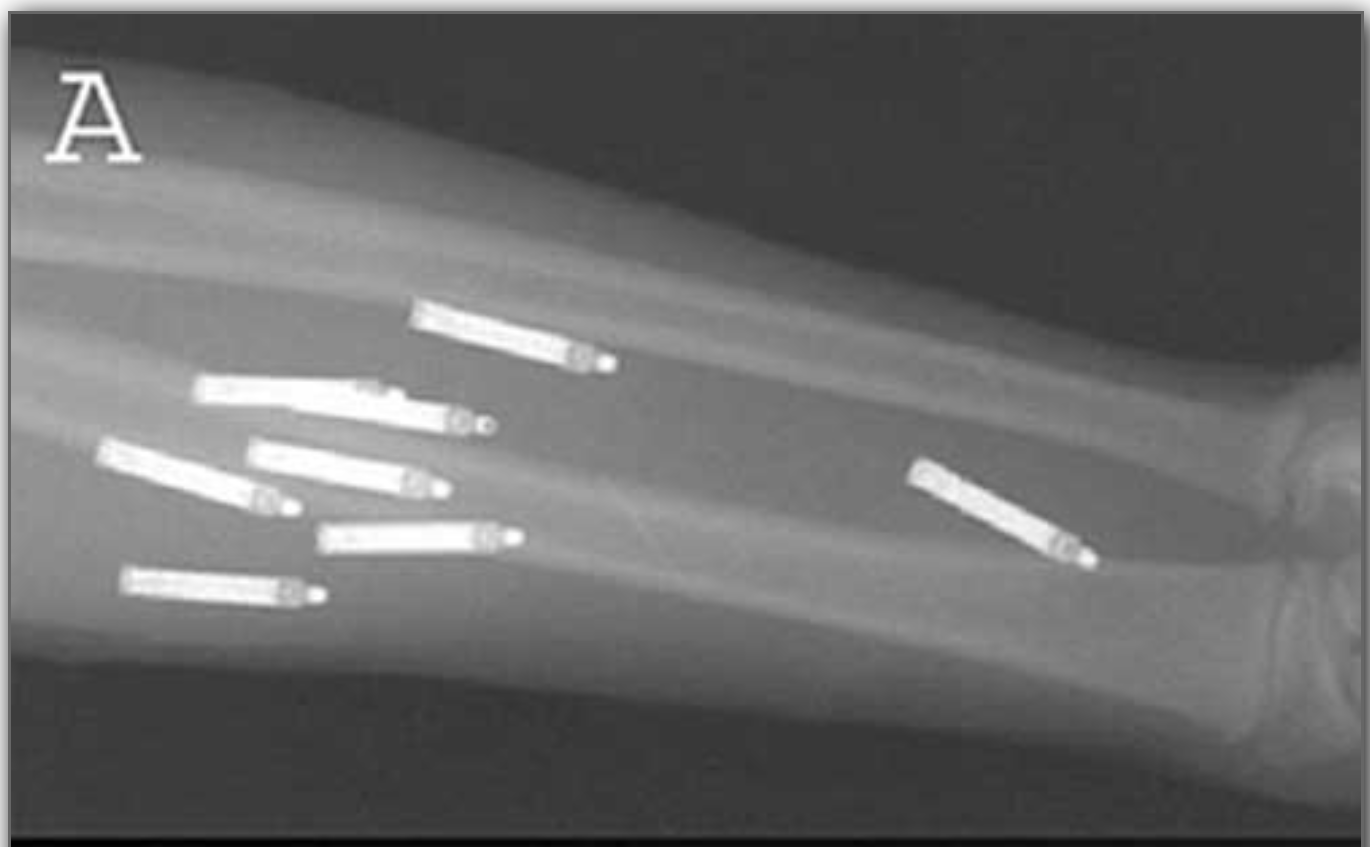
\includegraphics[width=0.75\textwidth]{figs/emg.png}
\caption{Implanted EMG electrodes \url{http://neural.iit.edu/research/imes/}}
\label{f:emg}
\end{figure}

Off the shelf electronics for surface EMG:\\
\url{http://www.advancertechnologies.com/p/muscle-sensor-v3.html}

\subsection{Operator muscle motion}

This implantable device measures relative motion of muscle relative
to other muscles and soft tissues:\\
\url{http://bme.usc.edu/assets/004/54640.pdf}

It would be relatively easy to develop implanted MEMs IMU devices (MEMs accelerometers
and gyros) to measure high frequency events (movement onset, reflexes,
impacts, relative muscle moition, muscle contraction, ...).\\
\url{http://www.designworldonline.com/surface-mount-accelerometer-for-implantable-medical-devices/}\\
\url{https://www.endevco.com/meggitt-sensing-systems-announces-endevco\%C2\%AE-surface-mount-accelerometer-series-for-implantable-medical-device-applications/}\\
\url{http://www.sciencedirect.com/science/article/pii/S0924424713005979}\\
\url{http://www.ncbi.nlm.nih.gov/pubmed/17574533}\\
\url{http://circep.ahajournals.org/content/3/6/657.full}\\

\subsection{Operator-exoskeleton force sensing}

Operator-exoskeleton forces may be measured (forcemyography (FMG))
with various types of
force sensors such as single and multi-axis strain-gage load cells,
force sensitive resistors (FSRs), and pressure sensors built into an internal exoskeleton skin or at the
contacts (straps and cushions) of the exoskeleton attachment points.
Optical sensors and other distance sensors can measure deformation and
strain of the operator and between the operator and the exoskeleton.
Overall muscle ``pressure'' and other tissue parameters can be measured using
elastic straps around the arm, deformation pressure probes at various
points on the arm.
An estimate of individual muscle activity
may be available from tissue impedance measurements on the arm
or through the arm (including various forms of reflective and transmissive
ultrasound imaging tracking tissue parameters or implanted markers).
Some or all operator-exoskeleton forces may not be measured, and must
be estimated with some sort of Kalman filter.
EMG and FMG can be usefully combined.

\url{http://ieeexplore.ieee.org/xpl/login.jsp?tp=&arnumber=6913842}\\

\begin{verbatim}
[8] K. Kong and M. Tomizuka, “A Gait Monitoring System Based on Air
Pressure Sensors Embedded in a Shoe,” IEEE/ASME Transactions on
Mechatronics, vol. 14, pp. 358–370, 2009.
\end{verbatim}

These devices measure relative motion of tissue, and could be used
to measure force by measuring tendon stretch:\\
\url{http://bme.usc.edu/assets/004/54640.pdf}

\subsection{Operator state and motion}

In a full-body exoskeleton
(not necessarily fully actuated), the
exoskeleton can be used to measure positions, velocities,
and accelerations. For partial exoskeletons,
it may be the case that additional sensors such as distributed 
angle sensors, tachometers, or inertial measurement units (IMUs)
are attached to or implanted in the operator 
or part of the operator's clothing.

\section{Modeling the individual operator}

We recommend each exoskeleton controller
to be used by and optimized for a single operator.
A substantial investment in capturing the operators normal behavior,
operator training and learning, and controller customization should be made.
This paper discusses ways to model individual movement style.\\
\url{http://humanmotion.ict.ac.cn/papers/2015P1_StyleTransfer/details.htm}\\
This paper discusses activity forecasting.\\
\url{http://www.ri.cmu.edu/publication_view.html?pub_id=7250}

Predictive models of human motion, a major topic of robot learning from\\
observation/demonstration/imitation and computer animation,
could be the subject of a future white
paper.\\
\url{http://ieeexplore.ieee.org/xpl/login.jsp?tp=&arnumber=6913830}\\
\url{http://www.ri.cmu.edu/publication_view.html?pub_id=7891}

\section{Can the operator help?}

We have a cooperative operator, who can signal using unused frequency
ranges or patterns on existing measurement
channels (brain signals, EMG, force, and motion) or use 
task specific interfaces such as built-in keyboards, touch sensors, joysticks,
and speech recognition.
Operators can resolve ambiguities, select behaviors, and indicate
parameterization (how far, how high, how fast) using these interfaces.

We note that the operator will probably use more command channels that just
body movement, since
the operator controls more than the pose and motion of the
exoskeleton. What if there are ``pointing'' sensors or communication
devices that need to be aimed at or track an area of interest? What if
there are additional (physical or virtual) pan/tilt/zoom cameras
pointing to the side and rear or line of sight secure communications,
for example. What about other controls, such as power assist level or
thermal control? It is an open question
how an operator can naturally express intent and
control these additional degrees of freedom.

\section{Conclusions and Recommendations}

1) We recommend using a Bayesian (probabilistic) framework for intent recognition
and prediction. This is similar to using an extended
Kalman filter and predictor for intent.
A classifying filter that tracks probabilities of different behavior selections
and their parameter selections can be implemented with a multiple model Kalman
filter or a particle filter.

2) We recommend developing an intent prediction system that can use
as many sensors and measurements of the operator as are possible within cost limits,
including at least external computer vision and audition, exoskeleton-world contact
force,
EMG, muscle pressure, force between the operator and the
exoskeleton,
speech acquisition, keyboards built into the exoskeleton handles or gloves,
and accelerometers/microphones/vibration-sensors attached to the operator skin.
This will enable the implementation of a variety of intent prediction approaches,
and avoid ``putting all our eggs in one basket.''

3) We seriously consider implanting devices and markers in operators.

4) We recommend each exoskeleton controller
to be used by and optimized for a single operator.
A substantial investment in capturing the operators normal behavior,
operator training and learning, and controller customization should be made.

\section{Appendix: Online Behavior Recognition}

\subsection{Review articles}

{\it 3D Gestural Interaction: The State of the Field,}\\
J. LaViola Jr.\\
\url{http://www.eecs.ucf.edu/~jjl/pubs/3dgesture.pdf}

\subsection{On-line (streaming) action recognition/detection in videos}

{\it Human Activity Prediction: Early Recognition of Ongoing Activities
from Streaming Videos,}\\
M. S. Ryoo\\
\url{http://michaelryoo.com/papers/iccv11_prediction_ryoo.pdf}

{\it Max-Margin Early Event Detectors,}\\
M. Hoai and F. De la Torre\\
\url{http://www.robots.ox.ac.uk/~minhhoai/papers/MMED_IJCV14.pdf}

\subsection{On-line (streaming) action recognition/detection using (Kinect) pose data}

{\it Exploring the Trade-off Between Accuracy and Observational Latency in
Action Recognition,}\\
C. Ellis, S. Z. Masood, M. Tappen, J. LaViola Jr., R. Sukthankar\\
\url{http://www.cs.ucf.edu/~mtappen/pubs/2012/ellis-et-al-ijcv-2012.pdf}

{\it The Moving Pose: An Efficient 3D Kinematic Descriptor for Low-Latency
Action Recognition and Detection,}\\
M. Zanfir, M. Leordeanu, C. Sminchisescu\\
\url{http://www.cv-foundation.org/openaccess/content_iccv_2013/papers/Zanfir_The_Moving_Pose_2013_ICCV_paper.pdf}

{\it Real-time Classification of Dance Gestures from Skeleton Animation,}\\
M. Raptis, D. Kirovski, H. Hoppe\\
\url{http://vision.ucla.edu/papers/raptisKH11.pdf}

\subsection{Accelerometer-based and other sensors}

{\it Activity Recognition on Streaming Sensor Data,}\\
N. Krishnan, D. Cook\\
\url{http://www.eecs.wsu.edu/~cook/pubs/pmc12.pdf}

{\it Macro-class Selection for Hierarchical kNN Classification of Inertial
Sensor Data,}\\
C. McCall, K. Reddy, M. Shah\\
\url{http://crcv.ucf.edu/papers/PECCS_2012.pdf}

{\it Audio-based Human Activity Recognition Using Non-Markovian Ensemble
Voting}\\
\url{http://www2.informatik.uni-freiburg.de/~spinello/storkROMAN12.pdf}

%\bibliographystyle{plain}
%\bibliography{exo}

\end{document}


